\documentclass[paper slide]{beamer}
\usetheme{Boadilla}
\usepackage{essay-def}
\usepackage{bm}
\usepackage{amsfonts}
\usepackage{amssymb}
\usepackage{amsmath}
\usepackage{amsthm}
\usepackage{comment}
\usepackage{subcaption}
\usepackage{geometry}
\usepackage{algorithmic}
\usepackage{algpseudocode}
\usepackage{algorithmicx}
\geometry{left=1cm,right=1cm}
    \title[Data-driven SGS modeling]{Data-driven subgrid-scale modeling for wall-bounded turbulence}
\author[J. Zhao]{Jiaxi Zhao \\ \small joint with S. Arisaka, Q. Li, T. Hasama, N. Ikegaya, W. Wang \\
\small NUS \& Kajima \& KU}
\date[\today]{The 19th OpenFOAM Workshop \\ \today}
\begin{document}
\par \setlength{\parindent}{2em}

\begin{frame}
\titlepage
\begin{figure}[ht]
	\centering
	\begin{subfigure}[b]{0.32\textwidth}
		
\includegraphics[width=.8\textwidth]{fig/nus-logo-horizon.png}
	\end{subfigure}
	\begin{subfigure}[b]{0.32\textwidth}
		
\includegraphics[width=.8\textwidth]{fig/kajima-logo.jpg}
	\end{subfigure}
	\begin{subfigure}[b]{0.32\textwidth}
		
\includegraphics[width=.8\textwidth]{fig/ku_logo.jpg}
	\end{subfigure}
\end{figure}
\end{frame}

\begin{frame}{Motivation:}
	\begin{itemize}
		\item 1. Performing DNS is unaffordable, even a LES with 50M grids of length 1000s takes several days.
		\item 2. Cheap simulation such as RANS and coarse-grid LES can not obtain accurate quantities such as peak pressure.
	\end{itemize}
	\begin{figure}[ht]
		\centering
		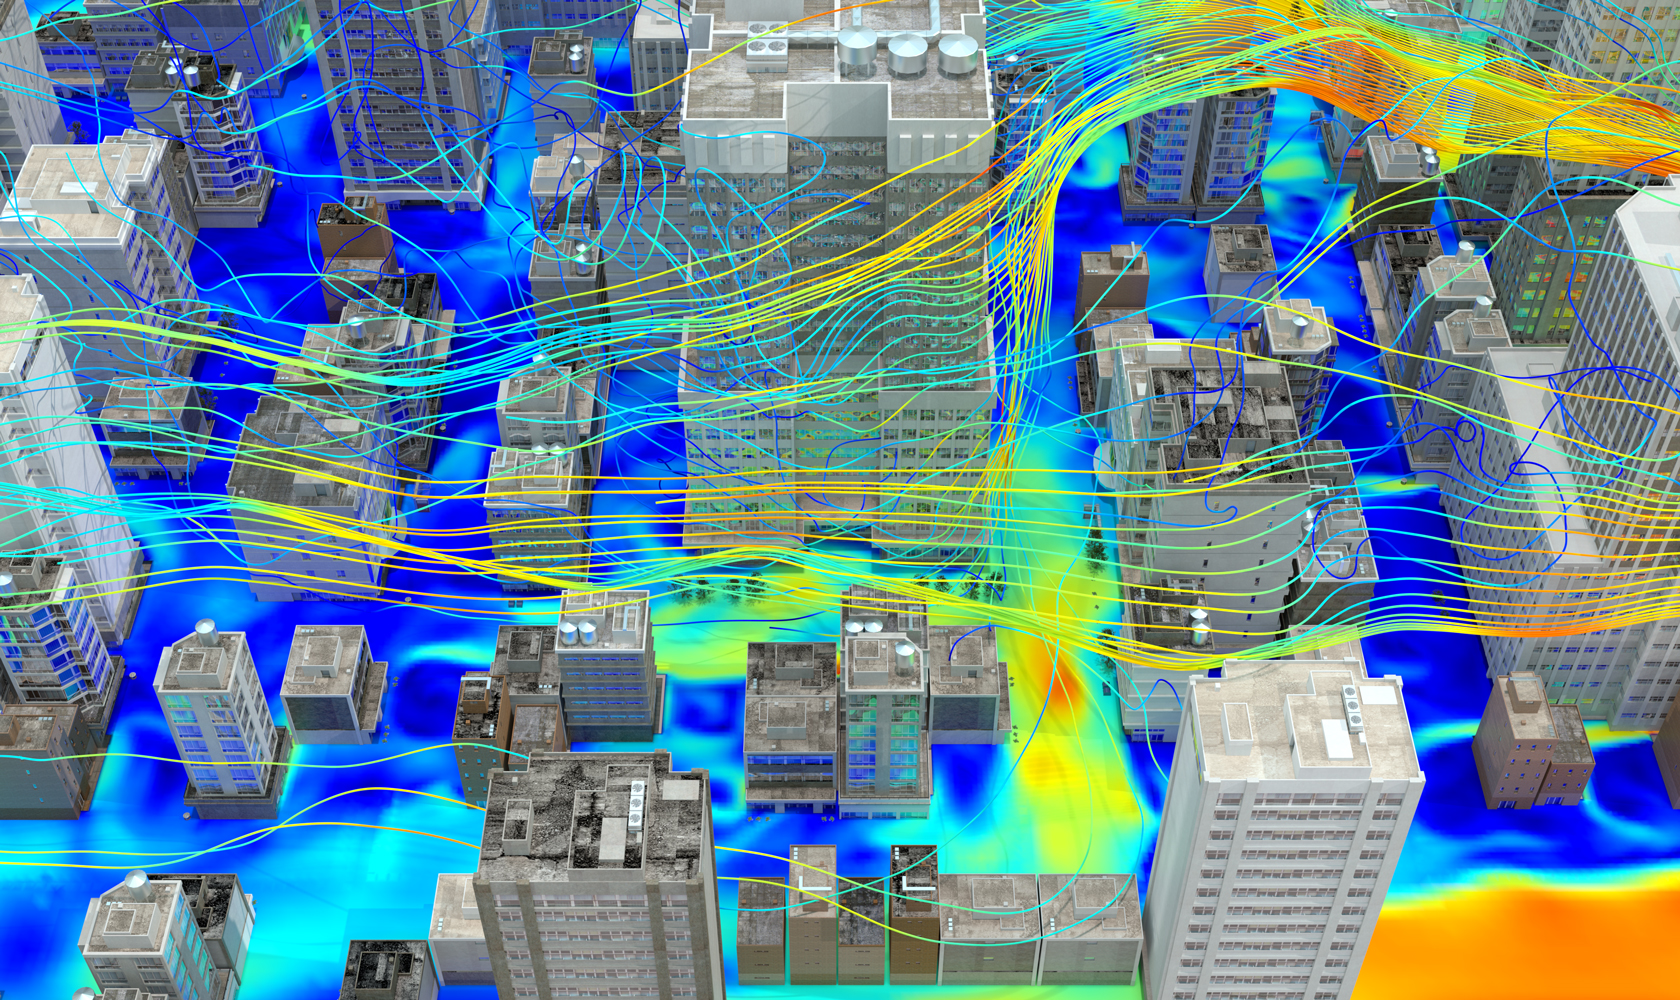
\includegraphics[width=.6\linewidth]{fig/urban_environment.jpeg}
	\end{figure}
	\textit{Can we {\color{red}design or learn better SGS models} based on the LES data so that it can achieve accurate
	results even {\color{red}on coarse grid LES?}}
\end{frame}

\begin{frame}{SGS stress modeling}
	There are three main issues for stress modeling:
	\begin{itemize}
		\item 1. The mapping from the input features. e.g. filtered velocity to the stress tensor is {\color{red}non-deterministic} while
		most classical turbulence models and data-driven models are deterministic.
		\begin{equation*}
			\overline{\mfU}, \nabla \overline{\mfU}, \overline{p} \overset{\text{NOT DETERMINISTIC}}{\Longrightarrow} \tau, \quad \min_{\phi}\norml \tau - \phi(\overline{\mfU}) \normr^2.
		\end{equation*}
		\item 2. Discrepancy between {\color{red}a-priori error and a-posteriori error}.
		\begin{equation*}
			\norml \wht\tau - \tau \normr^2, \quad \norml \overline{\wht\mfU}(T) - \overline{\mfU}(T) \normr^2
		\end{equation*}
		\item 3. Difficult to combine the OpenFOAM solver with gradient-based optimization algorithms.
	\end{itemize}
\end{frame}

\begin{frame}{Learning the SGS stress model}
	We test the following three approaches:
	\begin{itemize}
		\item 1. {\color{red}Directly predict} the stress tensor from the input features.
		\begin{equation}
			\tau = \text{NN}(\overline{\mfU}, \nabla \overline{\mfU}, \overline{p}).
		\end{equation}
		\item 2.  {\color{red}Learn a correction} of the constants to the Smagorinsky model.
		\begin{equation}
			\wtd C = \text{NN}(\overline{\mfU}, \nabla \overline{\mfU}, \overline{p}) + C, \quad \nu_t = \wtd C \Delta^2 \lv \bar{S} \rv.
		\end{equation}
		\item 3. Learn a  {\color{red}conditional generative model} from the input features.
	\end{itemize}
	\begin{itemize}
		\item The first approach usually provides a much better a-priori error estimate than the second approach.
	\end{itemize}
\end{frame}

\begin{frame}{Probabilistic SGS stress modeling}
	While the first two deterministic stress model can not capture the statistical behavior of the SGS stress,
	our probabilistic stress model manages this:
	\begin{figure}[ht]
		\centering
		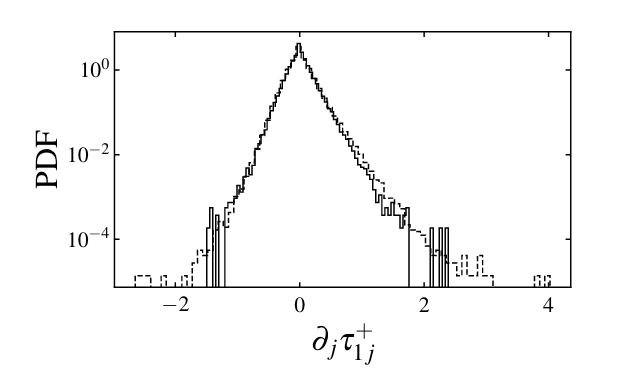
\includegraphics[width=.6\linewidth]{fig/stress_hist.jpg}
	\end{figure}
	\begin{figure}[ht]
		\centering
		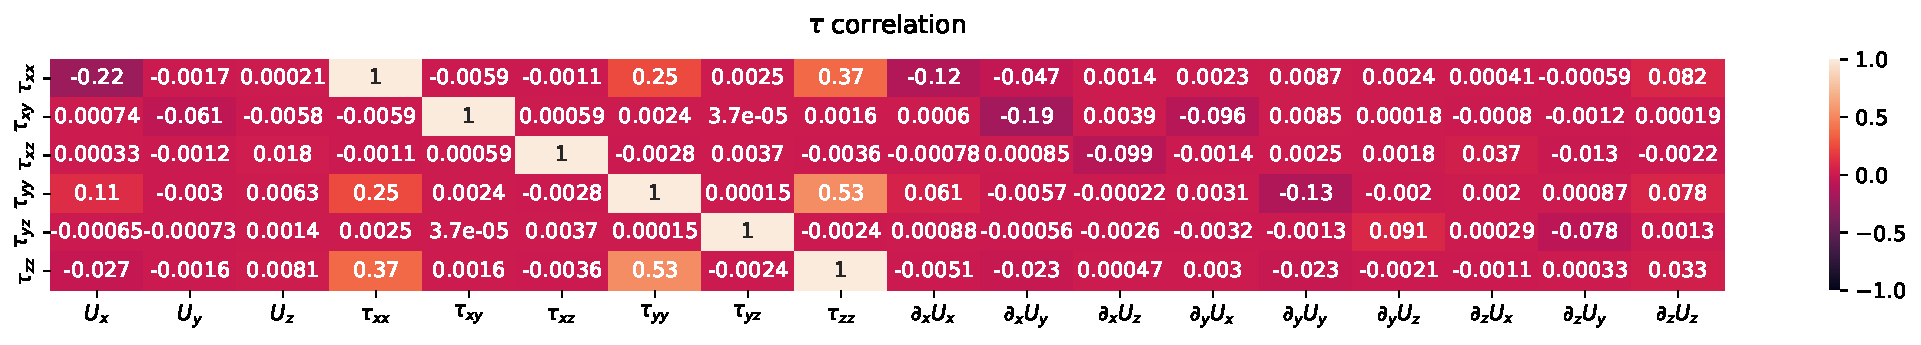
\includegraphics[width=1.2\linewidth]{fig/heatmap_tau.pdf}
	\end{figure}
\end{frame}

\begin{frame}{A-priori and a-posteriori discrepancy}
	The inconsistency between the a priori error and a posteriori error arises because the {\color{red}training algorithm does not take the solver dynamics into account}.
	\begin{figure}
		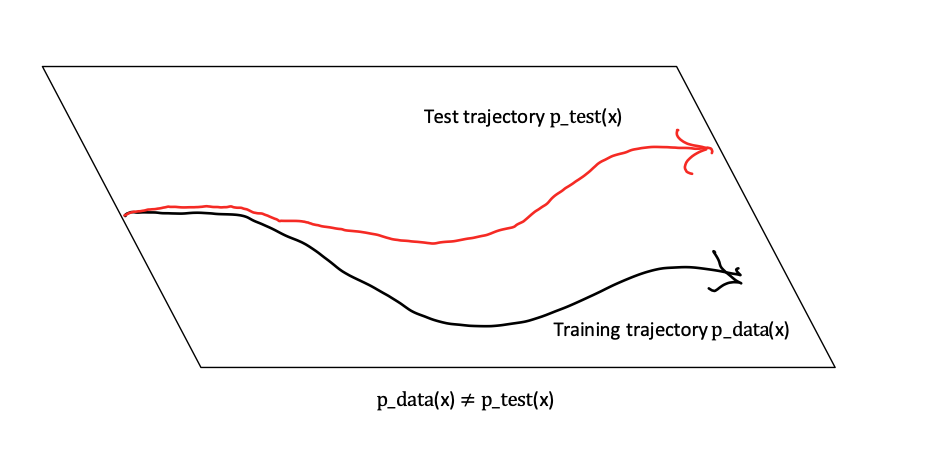
\includegraphics[width=.6\textwidth]{fig/dilemma.png}
		\label{fig:dilemma}
	\end{figure}
	The a-priori and a-posteriori performance are not consistent.
	\begin{figure}
		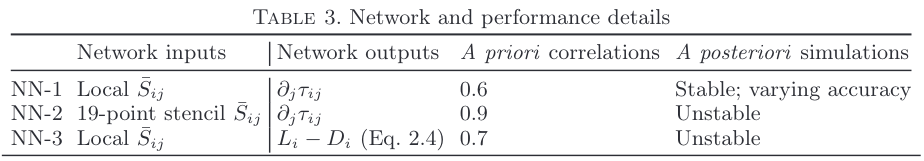
\includegraphics[width=.8\textwidth]{fig/dichotomy.jpg}
		\label{fig:dichotomy}
	\end{figure}
\end{frame}

\begin{frame}{A toy case}
	In a preliminary work, we apply {\color{red}tangent-space regularized method} to solve the NS equation using the projection
	method. 
	\bequn
		\begin{aligned}
			\mfu_{k+1} 	& = \mfu_k +
			\Delta t (\nu \Delta \mfu_k
			- (\mfu_k \cdot \nabla)\mfu_k - \nabla p_{k}),    \\
			p_{k} & = \phi(\mfu_k) = \Delta^{-1}(\nabla \cdot \lp \nu \Delta \mfu_k
			- (\mfu_k \cdot \nabla)\mfu_k\rp),   \\
		\end{aligned}
	\eequn
	Instead of training the data-driven model to solely	minimizing the a-priori error, we incorperate
	{\color{red}dynamical information, i.e. the iteration of the solver} into the algorithm that accounts for a-posteriori error.

	{\color{blue}For fluid people, this part needs more time to explain, I skip most of the details this time.}
\end{frame}

\begin{frame}{A toy case\footnotemark}
	\begin{figure}[ht]
		\centering
			\begin{subfigure}[b]{0.36\textwidth}
				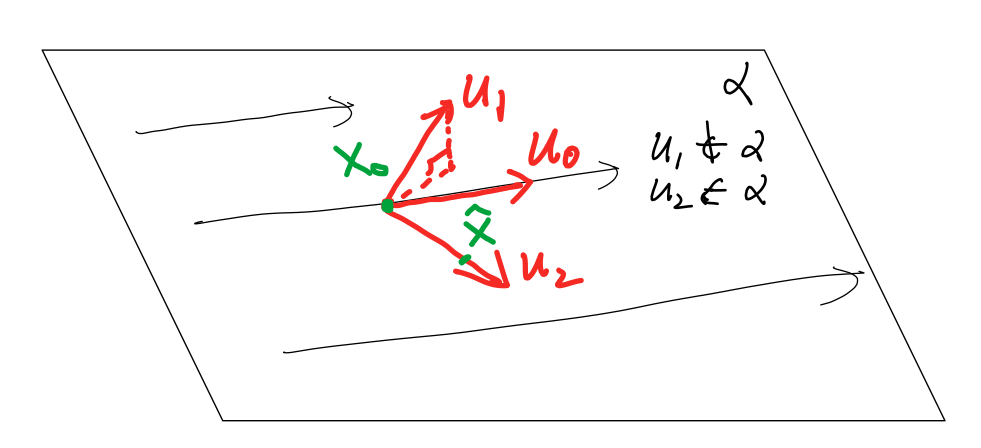
\includegraphics[width=\textwidth]{fig/mfd.png}
			\end{subfigure}
			\begin{subfigure}[b]{0.60\textwidth}
				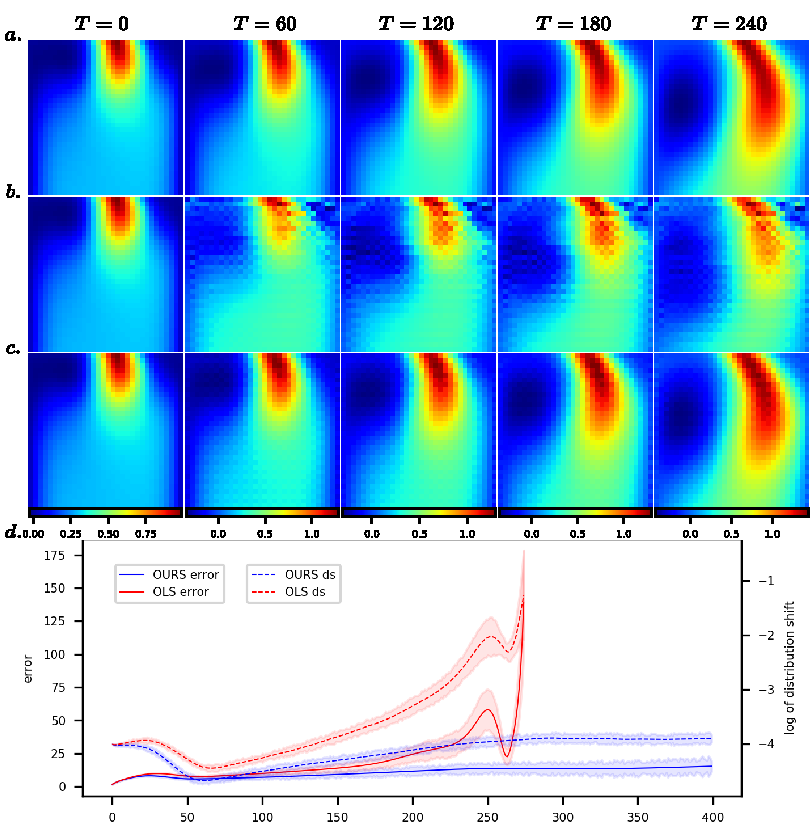
\includegraphics[width=\textwidth]{fig/NS-TR.pdf}
			\end{subfigure}
	\end{figure}
	\footnotetext[1]{J. Zhao and Q. Li (2024), Mitigating Distribution Shift in Machine Learning-augmented Hybrid Simulation, https://arxiv.org/pdf/2401.09259}
\end{frame}

\begin{frame}{Problem: Non-automatic-differentiable Solver}
    To directly minimize a posteriori error,
    we need to incorporate OpenFOAM solvers into the neural network training.
 
    However, they are not automatic-differentiable,
    and computing gradients through them is not trivial.
 
    \begin{figure}
        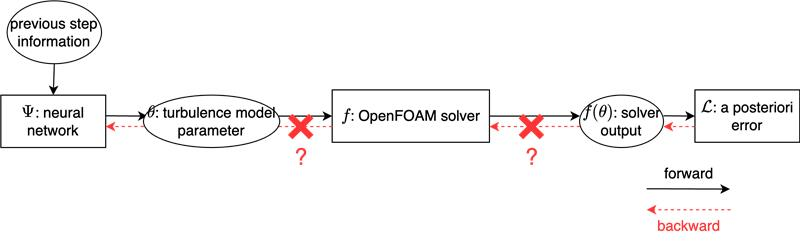
\includegraphics[width=\linewidth]{fig/of_problem.jpg}
    \end{figure}
    
\end{frame}
 
\begin{frame}{Solution: Non-intrusive Wrapper}
    To enable joint training with neural networks and such solvers,
    we developed a non-intrusive methodolgy that wraps the solvers
    to be compatible with neural network training.
 
    The key idea\footnotemark is to construct an unbiased and low-variance gradient estimator
    using a surrogate model that mimics the solver behavior.
 
    \begin{figure}
        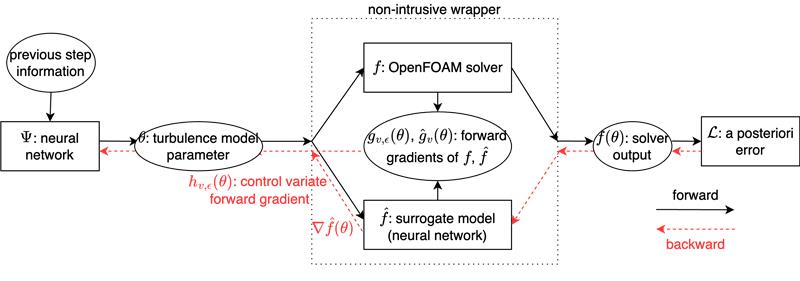
\includegraphics[width=\linewidth]{fig/of_solution.jpg}
    \end{figure}
    \footnotetext{S. Arisaka and Q. Li (2024) Accelerating Legacy Numerical Solvers by Non-intrusive Gradient-based Meta-solving}
    
\end{frame}


\begin{frame}{Preliminary result}
    We have applied the methodology to PETSc linear solver for Poisson equations by learning initial guesses
    and reduced the number of iterations by 74\%.
 
    We plan to apply it to learning turbulence models in OpenFOAM beyond linear solvers.
 
    \begin{figure}
        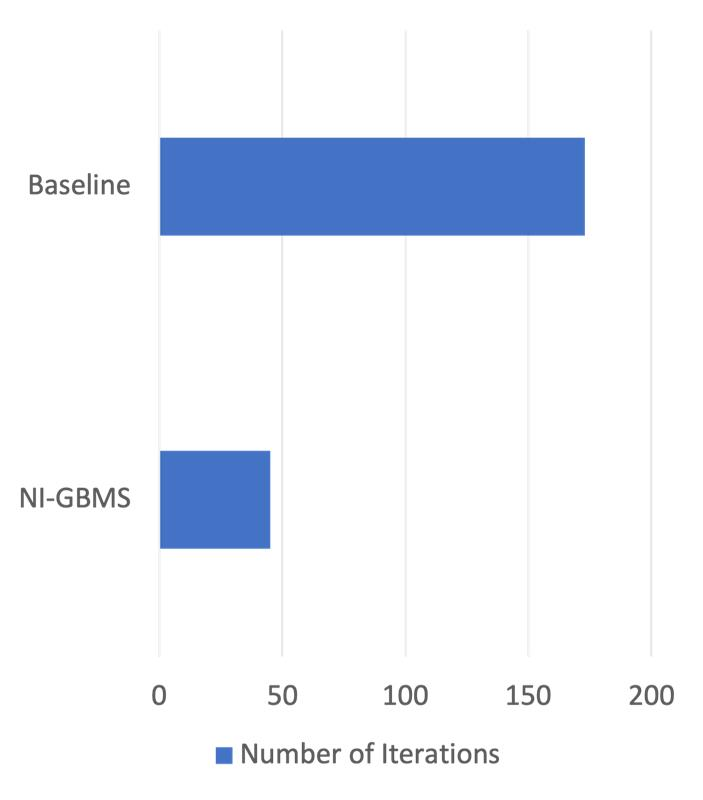
\includegraphics[width=0.4\linewidth]{fig/poisson_eq.jpg}
    \end{figure}    
    
\end{frame}
 

\begin{frame}{Future work}
	\begin{itemize}
		\item 1. Generate a systematical dataset of the flow around bluffs; train SGS models within the dataset and design algorithms
		which improves the a-posteriori performance.
		\item 2. Deploy to practical problems: Subgrid-scale modeling in large eddy simulation of the
		urban environment.
		\item 3. Investigate the statistical and numerical properties of the data-driven turbulence modeling, with
		special focus on the dataset characteristic and the relation between data with different resolution.
	\end{itemize}
\end{frame}

\begin{frame} % Use [allowframebreaks] to allow automatic splitting across slides if the content is too long
    \frametitle{References}
 
    \begin{thebibliography}{99} % Beamer does not support BibTeX so references must be inserted manually as below, you may need to use multiple columns and/or reduce the font size further if you have many references
        \footnotesize % Reduce the font size in the bibliography
 
		\bibitem[BDI]{bdi}
		M. Benjamin, S. Domino, and G. Iaccarino
		\newblock Neural Networks for Large Eddy Simulations of Wall-bounded Turbulence: Numerical Experiments and Challenges
		\newblock \emph{The European Physical Journal E}

		\bibitem[Zhao 2024]{ds}
        J. Zhao and Q. Li (2024)
        \newblock Mitigating Distribution Shift in Machine Learning-augmented Hybrid Simulation
        \newblock \emph{Arxiv preprint https://arxiv.org/pdf/2401.09259}

        \bibitem[S.A. and Q.L., 2024]{nigbms}
        S. Arisaka and Q. Li (2024)
        \newblock Accelerating Legacy Numerical Solvers by Non-intrusive Gradient-based Meta-solving
        \newblock \emph{International Conference on Machine Learning 2024}
 
        
    \end{thebibliography}
\end{frame}

\begin{comment}
\begin{frame}{Dataset generation}
	
\end{frame}

\begin{frame}{Dataset preprocessing}
	We analyze the distribution of different features in the dataset
	\begin{figure}
		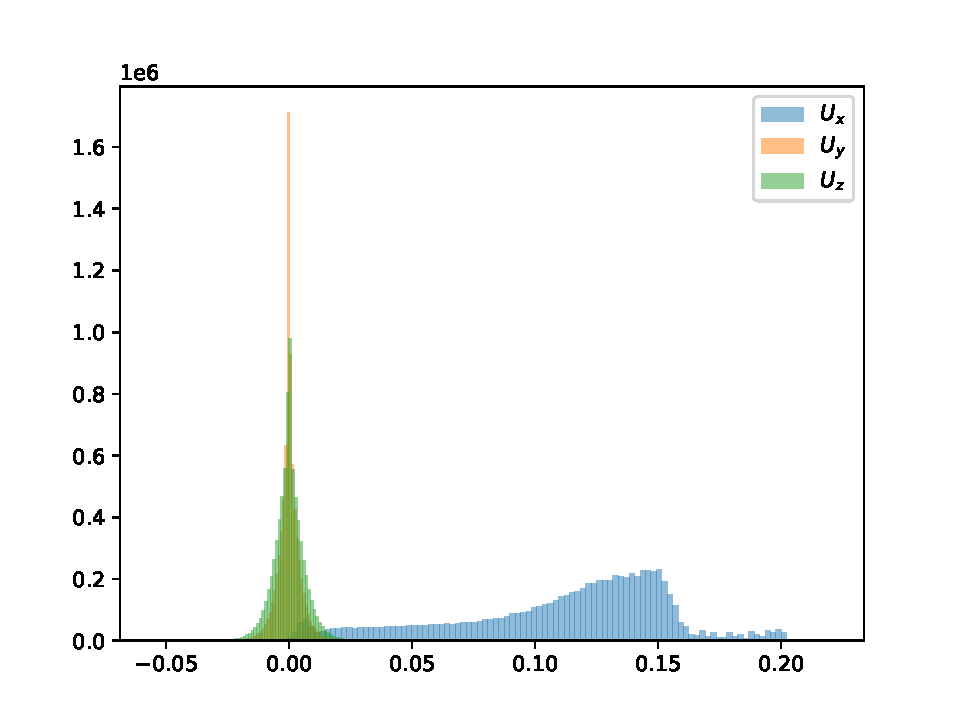
\includegraphics{fig/U_hist.pdf}
		\label{fig:U_hist}
		\caption{Histogram plot of the velocity magnitude $U$}
	\end{figure}
\end{frame}

\begin{frame}{Dataset difference}
	The a-priori test does not show a big difference between training with different datasets.
\end{frame}
\end{comment}

\end{document}